\documentclass[russian,utf8,emptystyle]{eskdtext}

\newcommand{\No}{\textnumero} % костыль для фикса ошибки

\ESKDdepartment{Федеральное государственное бюджетное образовательное учреждение высшего профессионального образования}
\ESKDcompany{Московский государственный технический университет им. Н. Э. Баумана}
\ESKDclassCode{23 0102}
\ESKDtitle{Лабораторная работа №3}
\ESKDdocName{по курсу <<Интеллектуальные системы>>}
\ESKDsignature{Решение задач с использованием искусственных нейронных сетей}
\ESKDauthor{Гуща~А.~В.}
\ESKDtitleApprovedBy{%
к.т.н., доцент}{Терехов~В.~И.}
\ESKDtitleAgreedBy{%
к.т.н., доцент}{Терехов~В.~И.}
\ESKDtitleDesignedBy{%
Студент группы ИУ5-82}{Гуща~А.~В}
 
\usepackage{multirow}
\usepackage{tabularx}
\usepackage{tabularx,ragged2e}
\renewcommand\tabularxcolumn[1]{>{\Centering}p{#1}}
\newcommand\abs[1]{\left|#1\right|}

\usepackage{geometry}
\geometry{footskip = 1cm}

\pagenumbering{arabic}
\pagestyle{plain}

\usepackage{listings}

\usepackage{xcolor}
\usepackage{listings}
\lstset{
    breaklines=true,
    postbreak=\raisebox{0ex}[0ex][0ex]{\ensuremath{\color{red}\hookrightarrow\space}},
    extendedchars=\true,
    %basicstyle=\tiny,
    inputencoding=utf8
}
\lstdefinelanguage{D}{
    keywords = {
    abstract,
    alias,
    align,
    asm,
    assert,
    auto,
    body,
    bool,
    break,
    byte,
    case,
    cast,
    catch,
    cdouble,
    cent,
    cfloat,
    char,
    class,
    const,
    continue,
    creal,
    dchar,
    debug,
    default,
    delegate,
    delete,
    deprecated,
    do,
    double,
    else,
    enum,
    export,
    extern,
    false,
    final,
    finally,
    float,
    for,
    foreach,
    foreach_reverse,
    function,
    goto,
    idouble,
    if,
    ifloat,
    immutable,
    import,
    in,
    inout,
    int,
    interface,
    invariant,
    ireal,
    is,
    lazy,
    long,
    macro,
    mixin,
    module,
    new,
    nothrow,
    null,
    out,
    override,
    package,
    pragma,
    private,
    protected,
    public,
    pure,
    real,
    ref,
    return,
    scope,
    shared,
    short,
    static,
    struct,
    super,
    switch,
    synchronized,
    template,
    this,
    throw,
    true, 
    try,
    typedef,
    typeid,
    typeof,
    ubyte,
    ucent,
    uint,
    ulong,
    union,
    unittest,
    ushort,
    version,
    void,
    volatile,
    wchar,
    while,
    with,
    __FILE__,
    __MODULE__,
    __LINE__,
    __FUNCTION__,
    __PRETTY_FUNCTION__,
    __gshared,
    __traits,
    __vector,
    __parameters,
    }
}

\begin{document}
\maketitle
\tableofcontents
\newpage

\pagenumbering{arabic}
\pagestyle{plain}

\section{Цель работы}
Целью лабораторной работы является углубление и закрепление теоретических знаний, полученных на лекциях, приобретение практических навыков самостоятельного исследования при решении задач выбора, обучения и работы ИНС.

В процессе выполнения лабораторной работы по теме «Решение задач с использованием искусственной нейронной сети» студенты решают следующие задачи (задания):
\begin{itemize}
\item описывают предметную область и выбирают решаемую задачу (предпочтение должно отдаваться задачам практической направленности);
\item определяют множество обучающих примеров;
\item в зависимости от решаемой задачи выбирают структуру ИНС;
\item выбирают алгоритм обучения ИНС;
\item проводят обучение ИНС на тестовом множестве примеров с помощью выбранного алгоритма обучения;
\item исследуют работу обученной ИНС в режиме распознавания.
\end{itemize}

\section{Задание}

Разработать программу, которая обучает ИНС распознавать прописные английские буквы на изображении любого размера и цвета, но состоящее не менее чем из 35 пикселей (матрица 5х7). При этом, ИНС должна иметь входы, ассоциированные с пикселями матрицы, и выходы, количество которых соответствует количеству прописных латинских букв.

В написанной или выбранной программе должна быть реализована возможность задания множества обучающих примеров в виде образов, а также изменения величины коэффициента скорости обучения. Программа должна предусматривать два режима работы: обучения и распознавания. Обучение должно производиться с использованием алгоритма, соответствующего архитектуре выбранной для решения задачи ИНС. Вероятность распознавания обученной ИНС должна быть не менее 65%.

\section{Описание предметной области и выбранной задачи}
Задача распознавания рукописного текста является одной из важнейших задач для интеллектуальных систем (распростаненная абвиатура OCR - optical character recognition). Успешное решение данной задачи применяется в следующих областях:
\begin{itemize}
\item оцифровка печатных книг, газет, журналов
\item автоматизированная обработка рукописных бланков
\item системы дополненной реальности
\end{itemize}

Входными данными являются растровые изображения рукописных (или печатных) символов прописных букв английского алфавита. Данные изображения имеют любой размер и цветовую информацию, но все изображения проходят предварительную обработку для изменения размера и бинаризации, чтобы данные изображения возможно было подать на вход разработанной ИНС. Ограничение на входные данные: прописные буквы должны быть вписаны в изображение, без наличия значительных пустых полей.

Выходными данными являются: распознанные символ и уверенность нейронной сети в данном ответе.

Искусственная нейронная сеть (ИНС) — математическая модель, а также её программная или аппаратная реализация, построенная по принципу организации и функционирования биологических нейронных сетей — сетей нервных клеток живого организма.

ИНС представляют собой систему соединённых и взаимодействующих между собой простых процессоров (искусственных нейронов). Такие процессоры обычно довольно просты (особенно в сравнении с процессорами, используемыми в персональных компьютерах). Каждый процессор подобной сети имеет дело только с сигналами, которые он периодически получает, и сигналами, которые он периодически посылает другим процессорам. И, тем не менее, будучи соединёнными в достаточно большую сеть с управляемым взаимодействием, такие локально простые процессоры вместе способны выполнять довольно сложные задачи.

\section{Структура, основные параметры выбранной ИНС}
Для решения данной задачи был выбран многослойный перцептрон, состоящий из четырех слоев: входного, выходного и двух скрытых. Каждый нейрон в слое $l$ имеет связи с каждым нейроном из слоя $l+1$.

Число нейронов в каждом слою:
\renewcommand{\theenumi}{\arabic{enumi}}
\begin{enumerate}
\item Соответствует количеству пикселей во входном бинарном изображении $5*7 = 35$
\item Размер данного слоя был выбран с учетом необходимости способности распознавать большое количество типов символов, исходя из практических наблюдений, размер первого скрытого слоя должен на порядок превышать входной: $35*35 = 1225$
\item Нейронны в данном слою отвечают за групировку сигналов из предыдущего слоя, в результате экспериментов был выбран размер в $35*2 = 70$ нейронов.
\item Каждый нейрон данного слоя соответствует одной букве английского алфавита: $26$
\end{enumerate}

Как функция активации используется сигмоида:
$$
F(x) = \frac{1}{1+e^{-x}}
$$

\begin{figure}[h!]

\includegraphics[width=0.9\textwidth]{neural-netowk-structure}
\caption{Структура ИНС}
\end{figure}
\clearpage

\subsection{Блок схема алгоритма обучения}
\begin{figure}[h!]
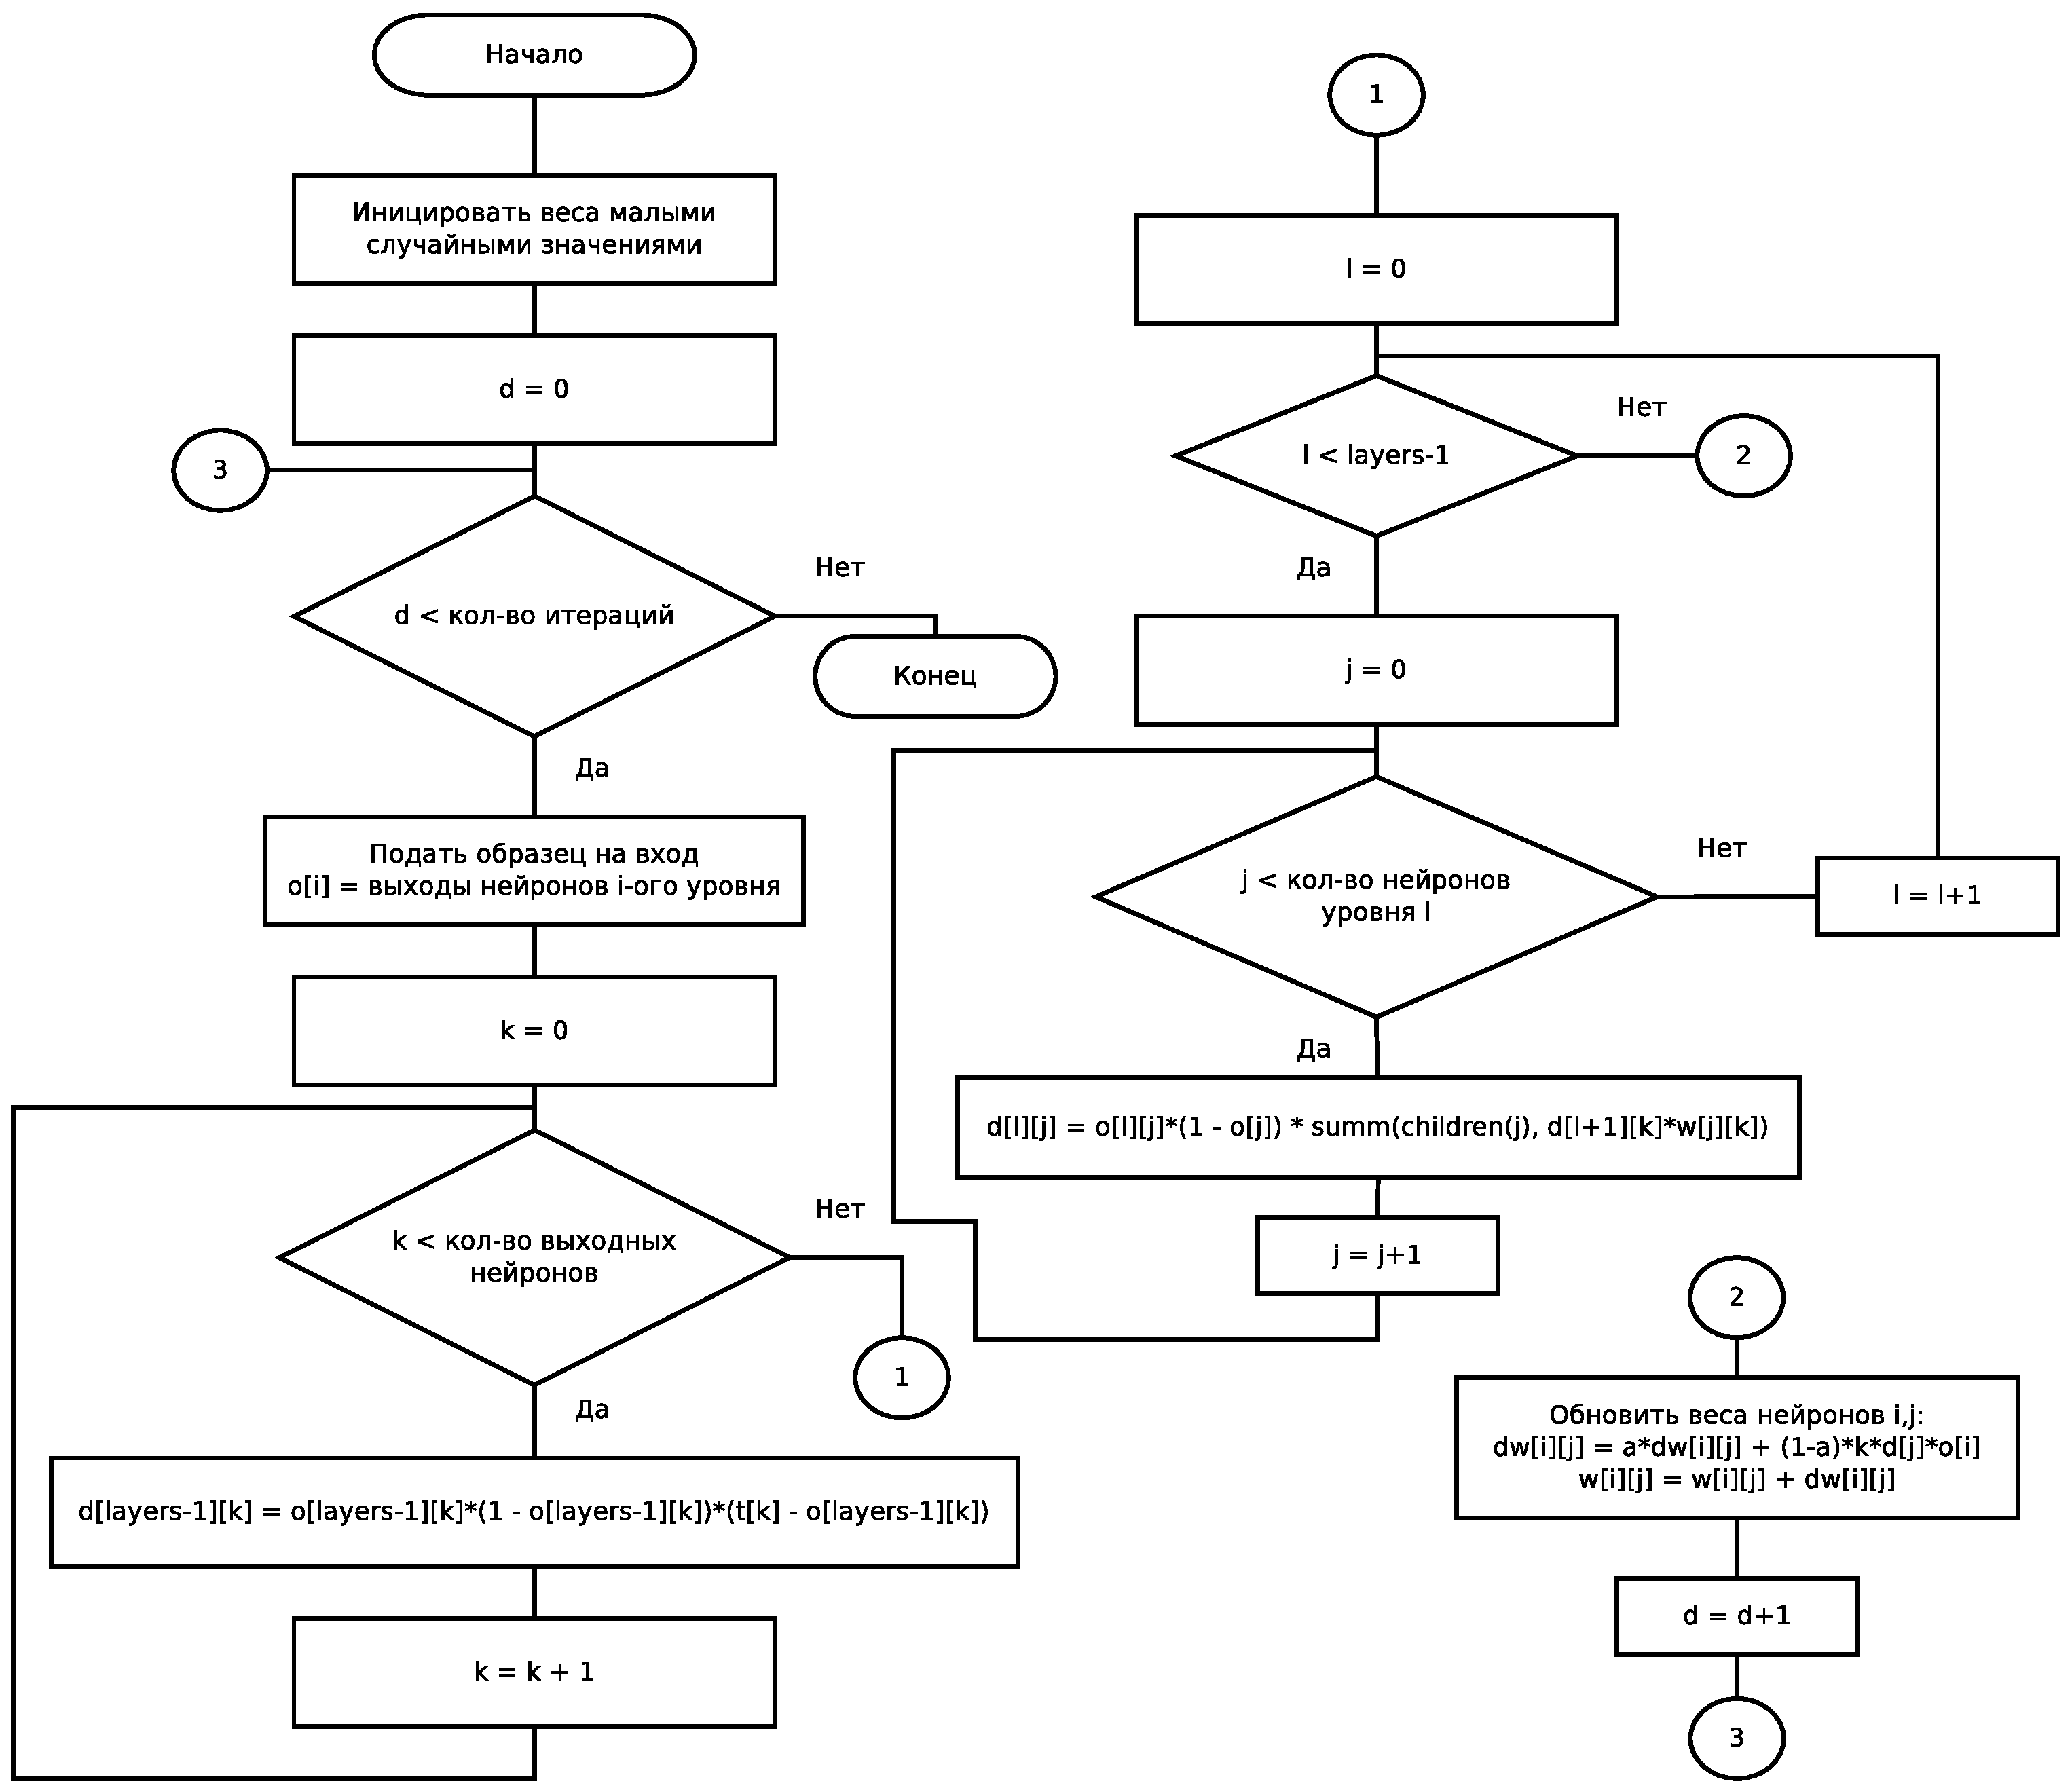
\includegraphics[width=1\textwidth]{train-algorithm}
\caption{Блок схема алгоритма обратного распространения ошибки}
\end{figure}
\clearpage

\section{Описание программы, ее ключевые особенности и новшества}
Одной из отличительной особенностью является предварительная обработка изображений:
\begin{itemize}
\item Исходное изображение преобразуется в изображение 5x7 пикселей
\item Проводится перевод цветовых каналов в серые тона
\item Бинаризация по критерию Оцу - позволяет разделить пиксели двух классов («полезные» и «фоновые»), рассчитывая такой порог, чтобы внутриклассовая дисперсия была минимальной.
\end{itemize}

Для обработки изображений был применен метод функциональной обработки изображений (и применена соответствующая библиотека, разработанная Владимиром Пантелеевым).
\begin{figure}[!htb]
\minipage{0.22\textwidth}

\includegraphics[width=\linewidth]{input-ex-source}
\caption{Исходное изображение}
\endminipage\hfill
\minipage{0.22\textwidth}

\includegraphics[width=\linewidth]{input-ex-resized}
\caption{Изменение размера}
\endminipage\hfill
\minipage{0.22\textwidth}

\includegraphics[width=\linewidth]{input-ex-grayscale}
\caption{Перевод в серые тона}
\endminipage\hfill
\minipage{0.22\textwidth}

\includegraphics[width=\linewidth]{input-ex-otsu}
\caption{Бинаризация по критерию Оцу}
\endminipage\hfill
\end{figure}

Все компонетны системы написаны на языке D - современный мультипарадигменный системный язык программирования. Исключительной особенностью является то, что архитектура нейронной сети задается на этапе компиляции. Генерация кода, описывающего ИНС, на этапе компиляции позволяет значительно оптимизировать скорость выполнения программы.
\clearpage
Пример генерации описания перцетрона, используемого в системе:
\begin{lstlisting}[language=D]
enum INPUT_SIZE_X = 5;
enum INPUT_SIZE_Y = 7;
enum INPUT_SIZE = INPUT_SIZE_X * INPUT_SIZE_Y;
enum OUTPUT_SIZE = 26;
alias TestNet = Perceptron!(INPUT_SIZE, INPUT_SIZE*INPUT_SIZE, 2*INPUT_SIZE, OUTPUT_SIZE);
\end{lstlisting}

Программа работает в консольном режиме, справку по пользованию программы можно получить, набрав в терминале команду:
\begin{verbatim}
$ perceptron --help
perceptron [args]

args: --learning    - defines learning mode for neural network
      --recognition - defines recognition mode for neural networ.
                      default flag.
      --config=path - configuration file, default is 'config.json'.
      --genconfig   - if set, new config file is generated in 
                      --config location + .example extention.
      --input       - test input to feed trained network. Default
                      is 'test.png'
\end{verbatim}

Программа может работать в двух режимах: режим обучения и режим распознавания. Все необходимые параметры для обучения и описание образоцов хранится в текстовом конфигруационном файле:
\begin{lstlisting}
{
	"recogintionFolder": "data/recognition",
	"recognitionSamples": [],
	"logFile": "perceptron.log",
	"learnFolder": "data/learn",
	"saveInput": false,
	"controlPart": "0.0",
	"networkFile": "network.json",
	"trainingFactor": "0.8",
	"inertiaFactor": "0.0",
	"iteratesCount": "50",
	"learnSamples": [
		{
			"path": "a",
			"symbol": "A"
		},
		{
			"path": "b",
			"symbol": "B"
		}
		... 
	]
}
\end{lstlisting}

\section{Протоколы проведенных экспериментов}
\subsection{Обучение сети}
Были подготовлены 260 обучающих изображений размером 50x70 пикселей каждый, по 10 изображений на каждую букву.

\begin{figure}[!htb]
\minipage{0.11\textwidth}

\includegraphics[width=\linewidth]{../data/learn/a/001}
\endminipage\hfill
\minipage{0.11\textwidth}

\includegraphics[width=\linewidth]{../data/learn/b/001}
\endminipage\hfill
\minipage{0.11\textwidth}

\includegraphics[width=\linewidth]{../data/learn/c/001}
\endminipage\hfill
\minipage{0.11\textwidth}

\includegraphics[width=\linewidth]{../data/learn/d/001}
\endminipage\hfill
\minipage{0.11\textwidth}

\includegraphics[width=\linewidth]{../data/learn/e/001}
\endminipage\hfill
\minipage{0.11\textwidth}

\includegraphics[width=\linewidth]{../data/learn/f/001}
\endminipage\hfill
\minipage{0.11\textwidth}

\includegraphics[width=\linewidth]{../data/learn/g/001}
\endminipage\hfill
\minipage{0.11\textwidth}

\includegraphics[width=\linewidth]{../data/learn/h/001}
\endminipage\hfill

\minipage{0.11\textwidth}

\includegraphics[width=\linewidth]{../data/learn/i/001}
\endminipage\hfill
\minipage{0.11\textwidth}

\includegraphics[width=\linewidth]{../data/learn/j/001}
\endminipage\hfill
\minipage{0.11\textwidth}

\includegraphics[width=\linewidth]{../data/learn/k/001}
\endminipage\hfill
\minipage{0.11\textwidth}

\includegraphics[width=\linewidth]{../data/learn/l/001}
\endminipage\hfill
\minipage{0.11\textwidth}

\includegraphics[width=\linewidth]{../data/learn/m/001}
\endminipage\hfill
\minipage{0.11\textwidth}

\includegraphics[width=\linewidth]{../data/learn/n/001}
\endminipage\hfill
\minipage{0.11\textwidth}

\includegraphics[width=\linewidth]{../data/learn/o/001}
\endminipage\hfill
\minipage{0.11\textwidth}

\includegraphics[width=\linewidth]{../data/learn/p/001}
\endminipage\hfill

\minipage{0.11\textwidth}

\includegraphics[width=\linewidth]{../data/learn/q/001}
\endminipage\hfill
\minipage{0.11\textwidth}

\includegraphics[width=\linewidth]{../data/learn/r/001}
\endminipage\hfill
\minipage{0.11\textwidth}

\includegraphics[width=\linewidth]{../data/learn/s/001}
\endminipage\hfill
\minipage{0.11\textwidth}

\includegraphics[width=\linewidth]{../data/learn/t/001}
\endminipage\hfill
\minipage{0.11\textwidth}

\includegraphics[width=\linewidth]{../data/learn/u/001}
\endminipage\hfill
\minipage{0.11\textwidth}

\includegraphics[width=\linewidth]{../data/learn/v/001}
\endminipage\hfill
\minipage{0.11\textwidth}

\includegraphics[width=\linewidth]{../data/learn/w/001}
\endminipage\hfill
\minipage{0.11\textwidth}

\includegraphics[width=\linewidth]{../data/learn/x/001}
\endminipage\hfill

\minipage{0.11\textwidth}

\includegraphics[width=\linewidth]{../data/learn/y/001}
\endminipage\hfill
\minipage{0.11\textwidth}

\includegraphics[width=\linewidth]{../data/learn/z/001}
\endminipage\hfill
\end{figure}

Обучение запускалось следующей коммандой:
\begin{verbatim}
$ ./perceptron --learning
\end{verbatim}

Обучение длилось около часа, ниже представлен график точности распознования на обучающей выборки в зависимости от времени:
\begin{figure}[h!]
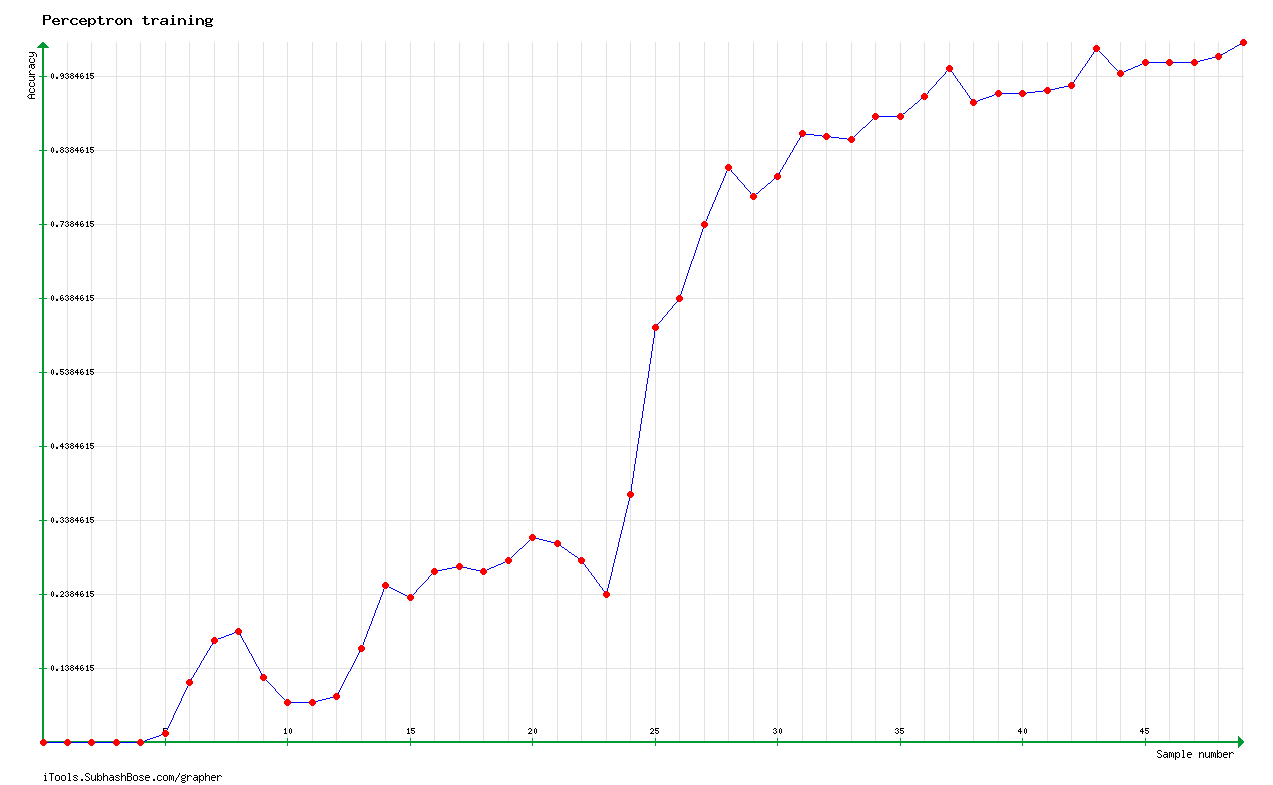
\includegraphics[width=1\textwidth]{perceptron_training}
\caption{График точности распознования во время обучения}
\end{figure}

В результате обучения удалось достичь точности распознования в $98.46 \%$ на обучающей выборке.

\subsection{Режим распознавания}
Для проверки обученной ИНС (и для практического использования) в программе присутствует режим распознования. Вызов режима распознования:

\begin{figure}[!htb]
\centering

\includegraphics[width=0.11\textwidth]{input-ex-source}
\caption{Входное изображение для тестирования ИНС my\_image.png}
\end{figure}

\begin{verbatim}
$ ./perceptron --recognition --input=my_image.png
Notice: Start initialization is finished
Notice: Application operates in recognition mode
Notice: Loading trained network from network.json
Notice: Loading test sample from test.png
Notice: Loading symbol map from config
Notice: Getting answer
Notice: Answer is: Y
Notice: Assurance is: 0.946363
\end{verbatim}

Программа выводит символ и уверенность сети в данном решении. В данном случае ответом является символ 'Y' и уверенность $94.64\%$

\clearpage
\section{Выводы}
В результате работы над лабораторной работы были усвоены следующие знания и навыки:
\begin{itemize}
\item Обработка изображений, изменение масштаба, бинаризация и фильтрация.
\item Постановка задачи в области OCR
\item Структура и логика работы многослойных ИНС, алгоритмы их обучения
\item Анализ работы ИНС, контроль процесса обучения
\item Навык скоростного рисования изображений прописных букв английского алфавита
\end{itemize}

В результате исследования работы ИНС после обучения было выявлены некоторые особенности выбранной архитектуры ИНС:
\begin{itemize}
\item Перцептрон не может распозновать изображения после сдвига, поворота, изменений масштаба.
\item ИНС может обрабатывать зашумленные данные на достойном уровне
\item Наиболее проблемной буквой является 'Q' из-за ее близости к букве 'O'. Стоить заметить, что частотное появление 'Q' в текстах на английском языке составляет всего $0,01\%$, что значительно понижает вероятность появления ошибки распознавания текстов.
\end{itemize}
\clearpage
\section{Используемая литература}
\renewcommand{\theenumi}{\arabic{enumi}}
\begin{enumerate}
\item Терехов В.И. Курс лекций по предмету <<Интеллектуальные системы>>, 2014
\item Wikipedia.org Искусственная нейронная сеть
\item Wikipedia.org Перцептрон
\item Wikipedia.org Метод обратного распространения ошибки
\item Wikipedia.org Метод Оцу
\item Vladimir Panteleev, Functional image processing in D
\end{enumerate}
\end{document}


